\documentclass[t]{beamer}

% packages
\usepackage[english]{babel}
\usepackage[utf8x]{inputenc}
\usepackage{mathtools}
\usepackage{amsfonts}
\usepackage{amsthm}
\usepackage{numprint}
\usepackage{amsxtra}
\usepackage{amsfonts}
\usepackage{graphicx}
\usepackage{color,colortbl}
\usepackage{enumerate}
\usepackage{booktabs}

% macros
% misc
\newcommand\todo[1]{\textcolor{red}{TODO: #1}}
\newcommand\hide[1]{\textcolor{white}{#1}}

% formatting
\newcommand\bld[1]{\textbf{#1}}
\newcommand\ul[1]{\underline{#1}}
\newcommand\n[1]{\numprint{#1}}
\newcommand{\ts}{\textsuperscript}
\newcommand\red[1]{\textcolor{red}{#1}}
\newcommand\blue[1]{\textcolor{blue}{#1}}
\newcommand\link[2]{\href{#1}{\textcolor{blue}{\underline{#2}}}}

% sets
\newcommand\set[1]{\mathcal{#1}}
\newcommand\bb[1]{\mathbb{#1}}
\renewcommand\:{\colon} % for use with \sset, etc.
\newcommand{\sset}[1]{\left\{\,#1\,\right\}} % { ? }, automatic brackets
\newcommand{\ssets}[1]{\left\{#1\right\}} % {?}, automatic brackets
\newcommand{\ssetn}[1]{\{\,#1\,\}} % { ? }, normal brackets

% table formatting
% To better align bold entries in S columns (still broken)
% \usepackage{siunitx}
% \robustify\bfseries
% \newrobustcmd{\bfcell}{\bfseries}

% vector variables (taken from macros by Rainer Gemulla)
\newcommand\vect[1]{{\boldsymbol{#1}}}
\newcommand\va{\vect{a}}
\newcommand\vb{\vect{b}}
\newcommand\vc{\vect{c}}
\newcommand\vd{\vect{d}}
\newcommand\ve{\vect{e}}
\newcommand\vf{\vect{f}}
\newcommand\vg{\vect{g}}
\newcommand\vh{\vect{h}}
\newcommand\vi{\vect{i}}
\newcommand\vj{\vect{j}}
\newcommand\vk{\vect{k}}
\newcommand\vl{\vect{l}}
\newcommand\vm{\vect{m}}
\newcommand\vn{\vect{n}}
\newcommand\vo{\vect{o}}
\newcommand\vp{\vect{p}}
\newcommand\vq{\vect{q}}
\newcommand\vr{\vect{r}}
\newcommand\vs{\vect{s}}
\newcommand\vt{\vect{t}}
\newcommand\vu{\vect{u}}
\newcommand\vv{\vect{v}}
\newcommand\vw{\vect{w}}
\newcommand\vx{\vect{x}}
\newcommand\vy{\vect{y}}
\newcommand\vz{\vect{z}}
\newcommand\vzero{\vect{0}}
\newcommand\vone{\vect{1}}

\newcommand\valpha{\vect{\alpha}}
\newcommand\vbeta{\vect{\beta}}
\newcommand\veps{\vect{\epsilon}}
\newcommand\vdelta{\vect{\delta}}
\newcommand\vtheta{\vect{\theta}}
\newcommand\vsigma{\vect{\sigma}}
\newcommand\vpi{\vect{\pi}}
\newcommand\vlambda{\vect{\lambda}}

% matrix variables (taken from macros by Rainer Gemulla)
\newcommand\mA{\vect{A}}
\newcommand\mB{\vect{B}}
\newcommand\mC{\vect{C}}
\newcommand\mD{\vect{D}}
\newcommand\mE{\vect{E}}
\newcommand\mF{\vect{F}}
\newcommand\mG{\vect{G}}
\newcommand\mH{\vect{H}}
\newcommand\mI{\vect{I}}
\newcommand\mJ{\vect{J}}
\newcommand\mK{\vect{K}}
\newcommand\mL{\vect{L}}
\newcommand\mM{\vect{M}}
\newcommand\mN{\vect{N}}
\newcommand\mO{\vect{O}}
\newcommand\mP{\vect{P}}
\newcommand\mQ{\vect{Q}}
\newcommand\mR{\vect{R}}
\newcommand\mS{\vect{S}}
\newcommand\mT{\vect{T}}
\newcommand\mU{\vect{U}}
\newcommand\mV{\vect{V}}
\newcommand\mW{\vect{W}}
\newcommand\mX{\vect{X}}
\newcommand\mY{\vect{Y}}
\newcommand\mZ{\vect{Z}}
\newcommand\mzero{\vect{0}}

\newcommand{\mPi}{{\ensuremath{\vect{\Pi}}}}
\newcommand{\mSigma}{{\ensuremath{\vect{\Sigma}}}}
\newcommand{\mLambda}{{\ensuremath{\vect{\Lambda}}}}

% argmin, argmax
\DeclareMathOperator*{\argmin}{argmin} % amsmath package required
\DeclareMathOperator*{\argmax}{argmax} % amsmath package required

% matrix operations
\newcommand\xdiag{\operatorname{diag}}      
\newcommand\diag[1]{\xdiag\left(#1\right)}    % diagonal matrix


% choose how your presentation looks.
% for more themes, color themes and font themes, see:
% http://deic.uab.es/~iblanes/beamer_gallery/index_by_theme.html

\mode<presentation>
{%
	\usetheme{default}      % or try Darmstadt, Madrid, Warsaw, ...
	\usecolortheme{default} % or try albatross, beaver, crane, ...
	\usefonttheme{default}  % or try serif, structurebold, ...
	\setbeamertemplate{navigation symbols}{}
	\setbeamertemplate{caption}[numbered]
	% For a numbered table of contents
	\setbeamertemplate{section in toc}[sections numbered] 
	% For slide numbers
	\addtobeamertemplate{navigation symbols}{}{%
	\usebeamerfont{footline}
	\usebeamercolor[fg]{footline}
	\hspace{1em}
	\insertframenumber%/\inserttotalframenumber
	}
} 

%% so table of content appears before each section, highlighting what's next
%\AtBeginSection[]
%{%
%	\setbeamercolor{section in toc shaded}{fg=structure}
%	\begin{frame}<beamer>
%	  \frametitle{Outline}
%	  \tableofcontents[currentsection]
%	\end{frame}
%}

% adds title slides for each section
\AtBeginSection[]{
  \begin{frame}
  \vfill
  \centering
  \begin{beamercolorbox}[sep=8pt,center,shadow=true,rounded=true]{title}
    \usebeamerfont{title}\Huge\insertsectionhead\par%
  \end{beamercolorbox}
  \vfill
  \end{frame}
}

\title[Write your short title here]{Advanced Methods in Text Analytics}
\subtitle{Exercise 02: DL Basics and Word Embeddings}
\author{Daniel Ruffinelli}
\institute{University of Mannheim}
\date{FSS 2025}

\begin{document}

% no "Figure X" prefix in image captions when using the figure environment
\setbeamertemplate{caption}{\raggedright\insertcaption\par}

\begin{frame}
    \titlepage{}
\end{frame}

\begin{frame}{Fully-Connected Neural Networks}{Context}
    \begin{itemize}
        \item An FNN is a compositional (possibly non-linear) function that
              transforms an input vector $\vx$ into a vector of outputs $\vy$.
        \item Each node is a unit that holds a numerical value.
        \item Each edge in the network also holds a numerical value.
        \item These units are combined to create \emph{layers}, usually an
              \emph{input} layer, an \emph{output} layer and any number of
              \emph{hidden} layers.
    \end{itemize}
    \vspace{0.5cm}
    \centering
    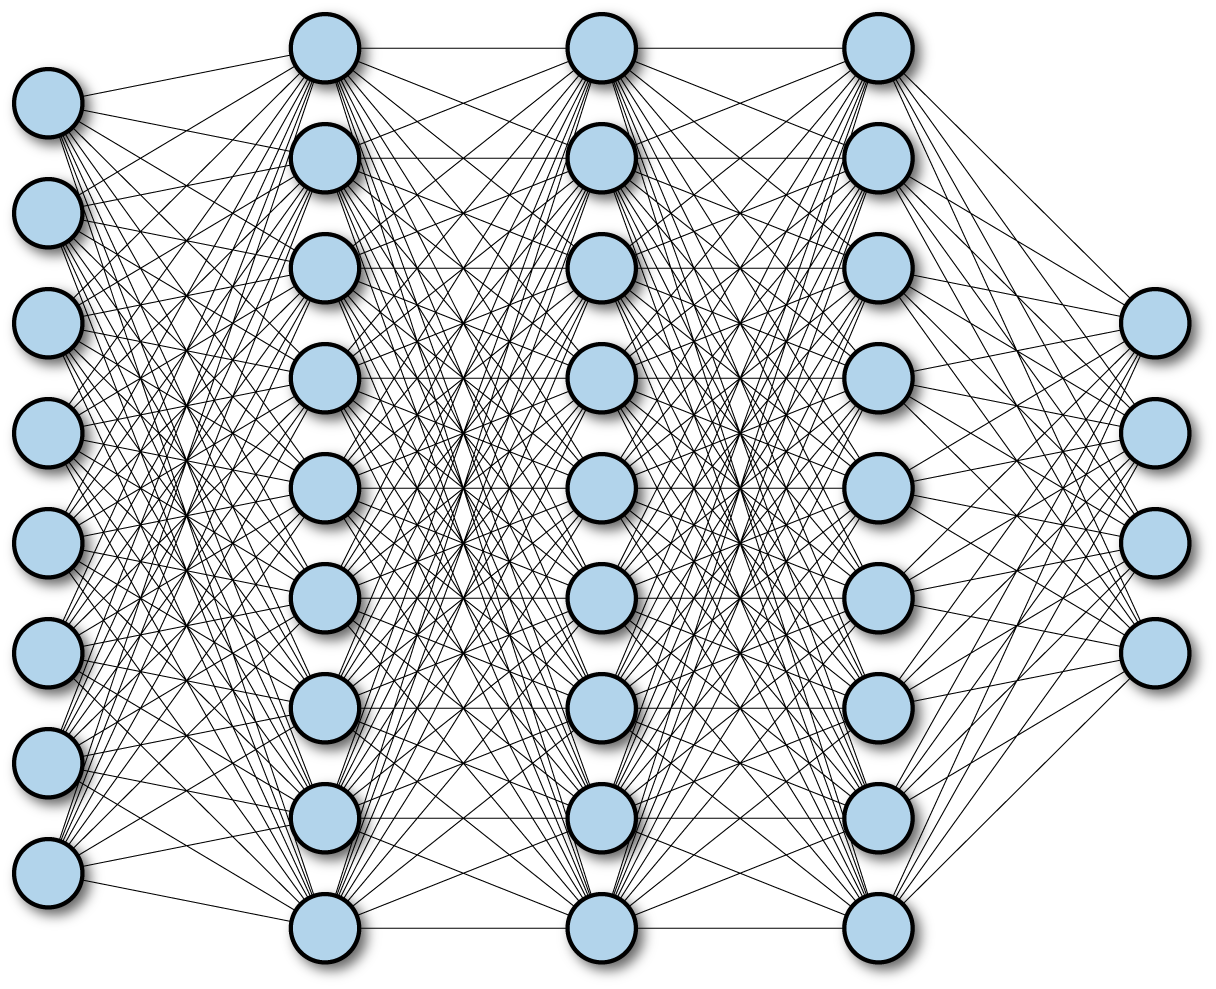
\includegraphics[scale=0.5]{img/fnn_1.png}
\end{frame}

\begin{frame}{Fully-Connected Neural Networks}{Question a)}
    \begin{itemize}
        \item \textbf{Question:} How many units should we have in the input
              layer? And in the output layer?
              \pause
        \item \textbf{Answer:} As many as we need, so $n$ input units, $m$
              output units, where $n$ is not necessarily equal to $m$.
    \end{itemize}
\end{frame}

\begin{frame}{Fully-Connected Neural Networks}{Question b)}
    \begin{itemize}
        \item \textbf{Question:} What is the difference between the values in
              nodes and those in edges?
              \pause
        \item \textbf{Answer:} Nodes hold values that are computed based on
              other nodes and some edges, whereas edges hold parameters of the
              function represented by the network.
    \end{itemize}
\end{frame}

\begin{frame}{Fully-Connected Neural Networks}{Question c)}
    \begin{itemize}
        \item What is the \emph{general} operation performed
              by each unit (node) in the network? What is the input to this
              operation? Give a formal expression for it.
    \end{itemize}
\end{frame}

\begin{frame}{Fully-Connected Neural Networks}{Answer c) (1)}
    \begin{itemize}
        \item Generally, the input of the operation computed by
              each node is the nodes from the previous layer
              \emph{that are connected to it by an edge.}
        \item The operation is a linear combination between the value in
              the input nodes and the corresponding weight vector $\vw_i$ made
              up of the values on the edges connecting the input vectors.
        \item Then, an \emph{activation} function $f$ is applied to the output
              of this linear combination.
        \item Concretely, let $h_i^{(k)}$ be the (output) value of the $i$-th
              unit in the $k$-th hidden layer in the network.
        \item We have:
              \begin{equation*}
                  h^{(k)}_i = f\left(\sum_{j=1}^{L^{k-1}}{h_j^{(k-1)} w_{i,j}^{(k)}}\right),
              \end{equation*}
              where $L^{k-1}$ is the size of the $(k-1)$-th layer and
              $w_{i,j}^{(k)}$ is the $j$-th component of $\vw_i$.
    \end{itemize}
\end{frame}

\begin{frame}{Fully-Connected Neural Networks}{Answer c) (2)}
    \begin{itemize}
        \item We can write this more compactly in vectorized form:
              \begin{equation*}
                  h^{(k)}_i = f(\vh_{(k-1)}^\top\vw_k),
              \end{equation*}
              where both $\vh,\vw$ are column vectors, $\vh_{(k-1)}$ is the
              vector with values in the $(k-1)$-th layer, and $f$ is applied
              element-wise.
    \end{itemize}
\end{frame}

\begin{frame}{Fully-Connected Neural Networks}{Question d)}
    \begin{itemize}
        \item \textbf{Question:} What is the main difference between different
              types of artificial neurons? Give two examples of different types
              of neurons.
              \pause
        \item \textbf{Answer:} The activation function. For example, ReLU,
              \emph{tanh}, the logistic function.
    \end{itemize}
\end{frame}

\begin{frame}{Fully-Connected Neural Networks}{Question e)}
    \begin{itemize}
        \item \textbf{Question:} Denote by $\mX\in\bb{R}^{N\times d}$ the input
              matrix constructed by stacking $N$ input vectors
              $\vx_i\in\bb{R}^d$ as rows. Similarly, denote by $\mH_1$ the
              matrix that contains the corresponding representations computed by
              the first hidden layer, which has $p$ units. What is the size of
              $\mH_1$? Give a formal expression for the operation that results
              in $\mH_1$ given input $\mX$.
              \pause
        \item \textbf{Answer:} $\mH_1=f(\mX\mW^T)\in\bb{R}^{N\times p}$ where
              $\mW\in\bb{R}^{p\times d}$ is the matrix constructed by stacking
              the weight vectors of each hidden unit in the first layer as rows,
              and $f$ is an activation function that is applied element-wise.
    \end{itemize}
\end{frame}

\begin{frame}{Backpropagation}{Context}
    \begin{itemize}
        \item With backpropagation, we can get gradient information that is
              useful to update the parameters of a multi-layer neural network
              during training.
        \item We start by computing the relevant gradients of the output layer
              and then continue backwards by computing the gradients of previous
              layers based on the gradients we computed before.
    \end{itemize}
\end{frame}

\begin{frame}{Backpropagation}{Question a)}
    \begin{itemize}
        \item {\textbf{Question:}} What are the \emph{relevant gradients} we
              care about during training?
              \pause
        \item \textbf{Answer:} $\frac{\partial}{\partial\vw}L$ where $L$ is our
              loss function and $\vw$ the model parameters we want to adjust
              during learning.
    \end{itemize}
\end{frame}

\begin{frame}{Backpropagation}{Question b)}
    \begin{itemize}
        \item The update rules of gradient-based optimizers require that we
              compute gradients of the functions we are optimizing.
        \item For example,
              when backpropagating through a layer with sigmoid activations, we
              will need the gradient of the sigmoid function.
        \item Show that this gradient is given by:
    \end{itemize}
    \begin{align*}
        \sigma(x)' & = \sigma(x) \cdot (1 - \sigma(x)), \text{where } \sigma(x) = \frac{1}{1 + e^{-x}}
    \end{align*}
\end{frame}

\begin{frame}{Backpropagation}{Answer b) (1)}
    \begin{itemize}
        \item We use standard derivation rules to get our result.
              \begin{align*}
                  \sigma(x)' & = \frac{d\sigma(x)}{d(x)}                                      \\
                             & = \frac{d(\frac{1}{1+e^{-x}})}{dx}                             \\
                             & = -\frac{1}{(1+e^{-x})^2}\cdot \frac{d(1+e^{-x})}{dx}          \\
                             & = -\frac{1}{(1+e^{-x})^2}\cdot (e^{-x}) \cdot \frac{d(-x)}{dx} \\
                             & = \frac{1}{(1+e^{-x})^2}\cdot (e^{-x})                         \\
                             & = \frac{e^{-x}}{(1+e^{-x})^2}                                  \\
                             & = \frac{1+e^{-x}}{(1+e^{-x})^2} - \frac{1}{(1+e^{-x})^2}       \\
              \end{align*}
    \end{itemize}
\end{frame}

\begin{frame}{Backpropagation}{Answer b) (2)}
    \begin{align*}
        \sigma(x)' & = \frac{1+e^{-x}}{(1+e^{-x})^2} - \frac{1}{(1+e^{-x})^2} \\
                   & = \frac{1}{(1+e^{-x})} - \frac{1}{(1+e^{-x})^2}          \\
                   & = \sigma(x)-\sigma(x)^2                                  \\
                   & = \sigma(x)\cdot (1-\sigma(x))
    \end{align*}
\end{frame}

\begin{frame}{Backpropagation}{Question c) (Context)}
    \begin{itemize}
        \item You are given a toy feed-forward neural network that predicts one
              of two classes given three input features: $x_1$, $x_2$,
              and $x_3$.
        \item The network has one hidden layer and one output layer, each
              consisting of two neurons.
        \item The activation function on both layers is
              the sigmoid function.
              \begin{center}
                  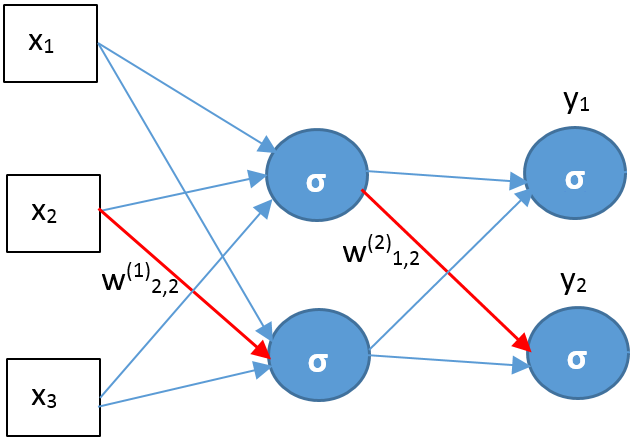
\includegraphics[scale=0.4]{img/backprop_2.png}
              \end{center}
    \end{itemize}
\end{frame}

\begin{frame}{Backpropagation}{Question c) (i)}
    \begin{itemize}
        \item Derive the update rule for the weights marked in red in the
              image, i.e., for $w^{(1)}_{2,2}$ and $w^{(2)}_{1,2}$.
        \item Assume you are training your model with the following square
              error loss:
              \begin{align*}
                  L & = -\frac{1}{2}\frac{1}{N}\sum_{e=1}^{N} \sum_{l=1}^{M} (t_{e,l}-y_{e,l})^2.
              \end{align*}
              where $N$ is size of the training set, $M$ is number of
              labels, $t_{e,l}$ the target label $l$ of example $e$ and
              $y_{e,l}$ the corresponding prediction made by the model.
        \item Note that in this toy setting, $M = N = 2$.
        \item Using square error loss for a classification task is not a
              common setting, but it is useful for us to construct a
              simple example to study backpropagation.
    \end{itemize}
\end{frame}

\begin{frame}{Backpropagation}{Question c) (ii)}
    \begin{itemize}
        \item You are given the toy dataset consisting of the following
              two training examples: $([-1, 0, 2], [0, 1])$ and
              $([2, 1, 1], [1, 0])$.
        \item These examples are of the form $(\vx, \vy)$, where $\vx$
              is input features, and $\vy$ is corresponding label.
        \item Assuming that all weights are initialized to $w = 1$, carry
              out one update iteration for denoted weights $w^{(1)}_{2,2}$
              and $w^{(2)}_{1,2}$, using the two training examples for
              supervision.
        \item Use learning rate $\psi = 1$ and the square error
              loss given above.
    \end{itemize}
\end{frame}

\begin{frame}{Backpropagation}{Answer c) (Some context)}
    \begin{itemize}
        \item In our setting, the network produces two numbers
              $y_1,y_2\in [0,1]$, each corresponding to the probability of one
              class.
        \item The given labels match this setting: a pair of binary numbers.
              E.g.\ label $[0,1]$ means the example corresponds to the 2nd
              class, not the first.
        \item Using squared error loss, we want the model to match its outputs
              to the given labels during training, so for label $[0,1]$, the
              model should match $y_1$ to 0 and $y_2$ to 1.
        \item This is achieved with the loss we were given:
              \begin{align*}
                  L & = -\frac{1}{2}\frac{1}{N}\sum_{e=1}^{N} \sum_{l=1}^{2} (t_{e,l}-y_{e,l})^2.
              \end{align*}
              where $N$ is the number of training examples (which we will keep
              as $N$ for clarity during derivations).
        \item Also, the $1/2$ factor simplifies computations, result unchanged.
    \end{itemize}
\end{frame}

\begin{frame}{Backpropagation}{Answer c) (i) (1)}
    \begin{itemize}
        \item Let $h_j$ be the value of hidden unit $j$, and
              $w_{i,j}^{(k)}$ the weight from input feature $i$ in layer
              $k-1$ to neuron $j$ in layer $k$.
              Our network architecture tells us that
              \begin{align*}
                  y_1 & = \sigma(w^{(2)}_{1,1}\cdot h_1 + w^{(2)}_{2,1}\cdot h_2)  \\
                  y_2 & = \sigma(w^{(2)}_{1,2}\cdot h_1 + w^{(2)}_{2,2}\cdot h_2).
              \end{align*}
        \item We derive the required gradient w.r.t. $w_{1,2}^{(2)}$ for
              the update rule as follows:
    \end{itemize}
\end{frame}

\begin{frame}{Backpropagation}{Answer c) (i) (2)}
    {\small
        \begin{align*}
            \frac{\partial L}{\partial w_{1,2}^{(2)}} & = - \frac{1}{2}\frac{1}{N}\sum_{e=1}^N \sum_{l=1}^2 \frac{\partial}{\partial w_{1,2}^{(2)}} \left(t_{e,l}-y_{e,l}\right)^2                                                                          \\
                                                      & = - \frac{1}{N} \sum_{e=1}^{N} \left( (-1)(t_{e,1}-y_{e,1})\cdot \frac{\partial y_{e,1}}{\partial w_{1,2}^{(2)}} + (t_{e,2}-y_{e,2}) \cdot \frac{\partial y_{e,2}}{\partial w_{1,2}^{(2)}}  \right) \\
                                                      & = - \frac{1}{N} \sum_{e=1}^{N} (t_{e,2}-y_{e,2})\cdot\frac{\partial y_{e,2}}{\partial w_{1,2}^{(2)}}                                                                                                \\
                                                      & = - \frac{1}{N} \sum_{e=1}^{N} (t_{e,2}-y_{e,2})\cdot y_{e,2}\cdot\left(1-y_{e,2}\right) \cdot \frac{\partial (w^{(2)}_{1,2}\cdot h_1 + w^{(2)}_{2,2}\cdot h_2)}{\partial w_{1,2}^{(2)}}            \\
                                                      & = - \frac{1}{N} \sum_{e=1}^{N} (t_{e,2}-y_{e,2})\cdot y_{e,2}\cdot\left(1-y_{e,2}\right) \cdot h_1
            = - \frac{1}{N} \sum_{e=1}^{N} \delta_{e,2} \cdot h_1,
        \end{align*}
        where $\delta_{e,2} = (t_{e,2}-y_{e,2})\cdot y_{e,2}\cdot\left(1-y_{e,2}\right).$
    }
\end{frame}

\begin{frame}{Backpropagation}{Answer c) (i) (3)}
    \begin{itemize}
        \item Similarly, our network architecture tells us that:
              \begin{align*}
                  h_1 & = \sigma(w^{(1)}_{1,1}\cdot x_1 + w^{(1)}_{2,1}\cdot x_2 + w^{(1)}_{3,1}\cdot x_3)  \\
                  h_2 & = \sigma(w^{(1)}_{1,2}\cdot x_1 + w^{(1)}_{2,2}\cdot x_2 + w^{(1)}_{3,2}\cdot x_3).
              \end{align*}
        \item Then, we obtain our gradient w.r.t. $w_{2,2}^{(1)}$ as follows:
    \end{itemize}
\end{frame}

\begin{frame}{Backpropagation}{Answer c) (i) (4)}
    {\small
        \begin{align*}
            \frac{\partial L}{\partial w_{2,2}^{(1)}} & = - \frac{1}{2N} \sum_{e=1}^N \sum_{l=2}^2 \frac{\partial}{\partial w_{2,2}^{(1)}} \left(t_{e,l}-y_{e,l}\right)^2                                                                                                                                                                                                                      \\
                                                      & = - \frac{1}{N} \sum_{e=1}^{N} \left( (t_{e,1}-y_{e,1})\cdot \frac{\partial y_{e,1}}{\partial w_{2,2}^{(1)}} + (t_{e,2}-y_{e,2}) \cdot \frac{\partial y_{e,2}}{\partial w_{2,2}^{(1)}}  \right)                                                                                                                                        \\
                                                      & = - \frac{1}{N} \sum_{e=1}^{N} \left( \delta_{e,1}\cdot\frac{\partial(w^{(2)}_{1,1}\cdot h_1 + w^{(2)}_{2,1}\cdot h_2)}{\partial w_{2,2}^{(1)}} + \delta_{e,2}\cdot\frac{\partial(w^{(2)}_{1,2}\cdot h_1 + w^{(2)}_{2,2}\cdot h_2)}{\partial w_{2,2}^{(1)}}  \right)                                                                   \\
                                                      & = - \frac{1}{N} \sum_{e=1}^{N} \left( \delta_{e,1}\cdot\frac{\partial w^{(2)}_{2,1}\cdot h_2}{\partial w_{2,2}^{(1)}} + \delta_{e,2}\cdot\frac{\partial w^{(2)}_{2,2}\cdot h_2}{\partial w_{2,2}^{(1)}}  \right)                                                     &  & \text{($\frac{\partial h_{1}}{\partial w_{2,2}^{(1)}} = 0$)} \\
                                                      & = - \frac{1}{N} \sum_{e=1}^{N} \left( \delta_{e,1}\cdot w^{(2)}_{2,1} \cdot h_2\cdot(1 - h_2)\cdot x_2 + \delta_{e,2}\cdot w^{(2)}_{2,2}\cdot h_2\cdot(1 - h_2)\cdot x_2  \right)                                                                                                                                                      \\
                                                      & = - \frac{1}{N} \sum_{e=1}^{N} \cdot h_2\cdot(1 - h_2)\cdot x_2 \sum_{l=1}^{2} \delta_{e,l}\cdot w^{(2)}_{2,l}.                                                                                                                                                                                                                        \\
        \end{align*}
    }
\end{frame}

\begin{frame}{Backpropagation}{Answer c) (i) (5)}
    \begin{itemize}
        \item We can now write our update rules for each of the weights:
              \begin{align*}
                  w_{1,2}^{(2)} & \coloneqq w_{1,2}^{(2)} + \frac{1}{N} \sum_{e=1}^{N} (t_{e,2}-y_{e,2})\cdot y_{e,2}\cdot\left(1-y_{e,2}\right) \cdot h_1             \\
                  w_{2,2}^{(1)} & \coloneqq w_{2,2}^{(1)} + \frac{1}{N} \sum_{e=1}^{N} \cdot h_2\cdot(1 - h_2)\cdot x_2 \sum_{l=1}^{2} \delta_{e,l}\cdot w^{(2)}_{2,l}
              \end{align*}
        \item Now all that is left is computing the forward pass and then
              applying our update rules to get our new weight values.
    \end{itemize}
\end{frame}

\begin{frame}{Backpropagation}{Answer c) (ii)}
    \begin{itemize}
        \item We compute our forward pass with $w^{(i)}_{j,k} = 1$ for all
              possible values of $i,j,k$ and the two given training
              examples:
              $\vx = \begin{pmatrix}
                      -1 \\
                      0  \\
                      2
                  \end{pmatrix}, \vh = \begin{pmatrix}
                      0.73 \\
                      0.73
                  \end{pmatrix}, \vy = \begin{pmatrix}
                      0.81 \\
                      0.81
                  \end{pmatrix}$ \qquad {\color{red} \text{Example 1}}
              $\vx = \begin{pmatrix}
                      2 \\
                      1 \\
                      1
                  \end{pmatrix}, \vh = \begin{pmatrix}
                      0.98 \\
                      0.98
                  \end{pmatrix}, \vy = \begin{pmatrix}
                      0.88 \\
                      0.88
                  \end{pmatrix}$ \qquad {\color{blue} \text{Example 2}}
        \item And our updates:
              {\tiny
              \begin{align*}
                  w_{1,2}^{(2)} & \coloneqq 1+ \frac{1}{2} ({\color{red} (1-0.81)\cdot 0.81 \cdot (1-0.81) \cdot 0.73} + { \color{blue}(0-0.88) \cdot 0.88 \cdot (1-0.88) \cdot 0.98}) \\
                                & \coloneqq 0.965                                                                                                                                      \\
                  w_{2,2}^{(1)} & \coloneqq 1+ \frac{1}{2} ({\color{red}0} + {\color{blue}1\cdot (1-0.98)\cdot 0.98 \cdot ((1-0.88)\cdot 0.88 \cdot (1-0.98) \cdot 1}                  \\
                                & \qquad\qquad\qquad\qquad\qquad\qquad\qquad\quad{\color{blue}+(0-0.88)\cdot0.88\cdot (1-0.98)\cdot 1)})                                               \\
                                & \coloneqq 0.99987.
              \end{align*}
              }
    \end{itemize}
\end{frame}

\begin{frame}{Skip-Gram Basics}{Context (1)}
    \begin{itemize}
        \item Consider the sentence
              \begin{align*}
                  \textit{The quick brown fox jumped over the lazy dog}, \\
                  c_1 \hspace{0.60cm}
                  c_2 \hspace{0.60cm}
                  w \hspace{0.60cm}
                  c_3 \hspace{0.80cm}
                  c_4 \hspace{2.35cm}
              \end{align*}
              where $w$ marks the \emph{center word} and $c_i$ the
              \emph{context words}.
        \item Here, we have a \emph{context window} of size $2$, meaning we use
              the 2 previous and 2 subsequent words around $w$ as context.
        \item In the lecture, skip-gram meant training a logistic regression
              model on the following binary classification task to learn word
              embeddings: $p(\text{True}|w,c) = \sigma{(l_{w,c})}$, where
              $l_{w,c}$ is the logit score (i.e.\ unnormalized prediction)
              produced by a logistic regression model given words $w$ and $c$.
        \item Given this task, sentence and context window, some positive
              examples of the form $(\text{source word}, \text{target word})$
              would be $(\textit{fox, quick})$, $(\textit{fox, brown})$, etc.
    \end{itemize}
\end{frame}

\begin{frame}{Skip-Gram Basics}{Context (2)}
    \begin{itemize}
        \item However, in their original work on the skip-gram approach, the
              authors learned word embeddings using a different task: predicting
              context word $c_j$ given center word $w_i$ in position $i$ of a
              given sequence of words.
        \item We refer to this task as the \emph{original task} throughout this
              exercise.
    \end{itemize}
\end{frame}

\begin{frame}{Skip-Gram Basics}{Question a)}
    \begin{itemize}
        \item How many classes are there in the original task proposed for
              skip-gram? And how could we compute probabilities for each class
              given logit scores from some classifier? Give a formal expression
              for this original task, including the way probabilities are
              computed from logits.
    \end{itemize}
\end{frame}

\begin{frame}{Skip-Gram Basics}{Answer a)}
    \begin{itemize}
        \item It's multi-class classification where the number of classes is the
              number of words in a given vocabulary $V$.
        \item We can describe the task with the expression $p(c_j|w_i)$.
        \item In such a setting, it's common to obtain probabilities using the
              softmax function.
        \item Formally, let $l_{w_i,c_j}$ be the logit score produced by a
              classifier trained for this task given center word $w_i$ and
              context word $c_j$.
        \item We then have:
              \begin{align*}
                  p(c_j|w_i) = \frac{\text{exp}{(l_{w_i,c_j}})}{\sum_{k\in V}\text{exp}(l_{w_i,c_k})},
              \end{align*}
              where $w_i$ is a word in position $i$ and $c_j$ is a word in a
              given context of size L, e.g.\ for L = 2, we have
              $j\in\{i-2, i-1,i+1,i+2\}$.
    \end{itemize}
\end{frame}

\begin{frame}{Skip-Gram Basics}{Question b)}
    \begin{itemize}
        \item Generate all positive training examples for the original skip-gram
              task using the given sentence above as the entire training set.
              Use a window size of 2.
    \end{itemize}
\end{frame}

\begin{frame}{Skip-Gram Basics}{Answer b) (1)}
    \begin{itemize}
        \item The sliding window moves through the sentence to create the
              following context windows:
              \begin{enumerate}
                  \item \colorbox{green!30}{The} \colorbox{yellow!30}{quick}  \colorbox{yellow!30}{brown} fox jumped over the lazy dog.
                  \item \colorbox{yellow!30}{The} \colorbox{green!30}{quick} \colorbox{yellow!30}{brown} \colorbox{yellow!30}{fox} jumped over the lazy dog.
                  \item \colorbox{yellow!30}{The} \colorbox{yellow!30}{quick} \colorbox{green!30}{brown} \colorbox{yellow!30}{fox} \colorbox{yellow!30}{jumped} over the lazy dog.
                  \item The \colorbox{yellow!30}{quick} \colorbox{yellow!30}{brown} \colorbox{green!30}{fox} \colorbox{yellow!30}{jumped} \colorbox{yellow!30}{over} the lazy dog.
                  \item The quick\colorbox{yellow!30}{brown} \colorbox{yellow!30}{fox} \colorbox{green!30}{jumped} \colorbox{yellow!30}{over} \colorbox{yellow!30}{the} lazy dog.
                  \item The quick brown \colorbox{yellow!30}{fox} \colorbox{yellow!30}{jumped} \colorbox{green!30}{over} \colorbox{yellow!30}{the} \colorbox{yellow!30}{lazy} dog.
                  \item The quick brown fox \colorbox{yellow!30}{jumped} \colorbox{yellow!30}{over} \colorbox{green!30}{the} \colorbox{yellow!30}{lazy} \colorbox{yellow!30}{dog}.
                  \item The quick brown fox jumped \colorbox{yellow!30}{over} \colorbox{yellow!30}{the} \colorbox{green!30}{lazy} \colorbox{yellow!30}{dog}.
                  \item The quick brown fox jumped over \colorbox{yellow!30}{the} \colorbox{yellow!30}{lazy} \colorbox{green!30}{dog}.
              \end{enumerate}
        \item Green marks center words, yellow marks context words
        \item The following table lists all examples generated for the original
              skip-gram task using a context window of size 2 and the given
              sentence.
    \end{itemize}
\end{frame}

\begin{frame}{Skip-Gram Basics}{Answer b) (2)}
    \centering
    \begin{tabular}{ccc}
        \toprule
        Context Window & Source Word & Target Word \\
        \midrule
        1              & The         & quick       \\
        1              & The         & brown       \\
        2              & quick       & The         \\
        2              & quick       & brown       \\
        2              & quick       & fox         \\
        3              & brown       & The         \\
        3              & brown       & quick       \\
        3              & brown       & fox         \\
        3              & brown       & jumped      \\
        4              & fox         & quick       \\
        4              & fox         & brown       \\
        4              & fox         & jumped      \\
        4              & fox         & over        \\
        \vdots         & \vdots      & \vdots      \\
        \bottomrule
    \end{tabular}
\end{frame}

\begin{frame}{Skip-Gram Basics}{Question c)}
    \begin{itemize}
        \item How is the skip-gram model parameterized? What is the role of each
              parameter?
        \item Assume your vocabulary consists of 101.425 words and you want to
              learn word representations of 300 dimensions each.
        \item What is the number of parameters in the skip-gram approach in this
              setting?
    \end{itemize}
\end{frame}

\begin{frame}{Skip-Gram Basics}{Answer c)}
    \begin{itemize}
        \item The skip-gram model learns two word vectors for each word in our
              vocabulary: one for when words are center (or source) words, and
              one for when words are context (or target) words.
        \item Let $\mW$ be the matrix constructed by stacking vectors of center
              representations as rows, and $\mW'$ the matrix constructed in the
              same way using context word representations.
        \item Then $\vtheta=\{\mW, \mW'\}$.
        \item The size of these matrices, and thus the number of parameters in
              our skip-gram model, for our given vocabulary and vector size is:
              \begin{align*}
                   & \mW\in\mathbb{R}^{101425\times 300}   \\
                   & \mW'\in\mathbb{R}^{101425\times 300}.
              \end{align*}
    \end{itemize}
\end{frame}

\begin{frame}{Skip-Gram Basics}{Question d)}
    \begin{itemize}
        \item Assume that word \textit{Frodo} is the 79th word in your
              vocabulary.
              How do we obtain a single (final) representation of the word
              \textit{Frodo} after our model has finished training?
              What decision do we need to make to obtain such a final
              representation?
    \end{itemize}
\end{frame}

\begin{frame}{Skip-Gram Basics}{Answer d)}
    \begin{itemize}
        \item We obtain vectors for a given word with a simple lookup function,
              i.e.\ a 1-to-1 mapping between words in our vocabulary and rows of
              $\mW$ and $\mW'$.
        \item To obtain a single (final) representation of a given word, we need
              to decide how to use the corresponding parameters in $\mW$ and
              $\mW'$.
        \item For example, we may discard the representations in $\mW'$ and
              simply use $\vw_{Frodo} = \mW_{79}$, i.e.\ the 79th row of matrix
              $\mW$.
        \item Or we may choose to concatenate the corresponding representations
              from $\mW$ and $\mW'$, i.e.
              $\vw_{Frodo} = \mW_{79}\oplus\mW'_{79}$.
        \item Instead of concatenation, one could also use other operations
              between vectors, such as computing the sum or average between the
              two.
        \item Concatenation is a safe operation in that it does not change the
              learned features, at the expense of doubling the dimension size of
              final vectors.
    \end{itemize}
\end{frame}

\begin{frame}{Skip-Gram Training}{Context}
    \begin{itemize}
        \item We now focus on how to train models using the skip-gram approach.
        \item  Assume throughout that we use dot products to compute logit
              scores, i.e. $l_{w_i,c_j} = \vw_i^T\vw'_j$, and that we use the
              softmax function to obtain probabilities from logit scores
    \end{itemize}
\end{frame}

\begin{frame}{Skip-Gram Training}{Question a)}
    \begin{itemize}
        \item To train a skip-gram model, we find the parameters $\vtheta$, i.e.
              word embedings, that maximize the likelihood of our training data,
              i.e.\ we perform MLE.
        \item Given text corpus $T$, give the expression for the dataset
              likelihood $L(\vtheta|T)$ as determined by a skip-gram model with
              a context window of size $L$.
        \item Give the corresponding negative log-likelihood expression under
              the empirical risk minimization framework.
        \item As in the lecture, assume independence between words and training
              examples (i.i.d. assumption)
    \end{itemize}
\end{frame}

\begin{frame}{Skip-Gram Training}{Answer a)}
    \begin{itemize}
        \item The likelihood of the entire text corpus $T$ with a context window
              of size $L$ is given by:
              \begin{align*}
                  L(\vtheta|T) = \prod_{t=1}^{|T|}\prod_{-L\leq j\leq L, j\neq 0} p(w_{t+j}|w_t,\vtheta).
              \end{align*}
        \item Note we assume all words are \emph{conditionally}
              independent of each other \emph{given} parameters $\vtheta$, i.e.\
              the embeddings.
        \item In other words, we assume the embeddings encode the dependencies
              between words.
        \item The corresponding negative log-likelihood function using empirical
              risk minimization is given by:
              \begin{align*}
                  \text{NLL}(\vtheta) = - \frac{1}{|T|} \sum_{t=1}^{|T|} \sum_{-L\leq j\leq L, j\neq 0} \log p(w_{t+j}|w_t,\vtheta).
              \end{align*}
        \item During training, we find the values of $\vtheta$ that minimize
              this expression using gradient-based optimizers.
    \end{itemize}
\end{frame}

\begin{frame}{Skip-Gram Training}{Question b)}
    \begin{itemize}
        \item Recall that computing the negative log-likelihood is equivalent to
              using cross-entropy loss.
        \item Consider the following toy vocabulary
              V=\{\textit{Daenerys}, \textit{Frodo}, \textit{ring}, \textit{dragon}, \textit{Picard}, \textit{ship}\}.
        \item Assume you are training a skip-gram model over a large corpus $T$
              with this vocabulary, and that the current values of the
              parameters of your model are the following:
              \[
                  \mathbf{W}=
                  \begin{bmatrix}
                      0.54 & 0.25 & 0.07 \\
                      0.91 & 0.74 & 0.27 \\
                      0.58 & 0.00 & 0.05 \\
                      0.16 & 0.77 & 0.31 \\
                      0.10 & 0.54 & 0.32 \\
                      0.59 & 0.99 & 0.06
                  \end{bmatrix},
                  \mathbf{W'}=
                  \begin{bmatrix}
                      0.19 & 0.64 & 0.98 \\
                      0.17 & 0.42 & 0.47 \\
                      0.55 & 0.24 & 0.92 \\
                      0.89 & 0.58 & 0.13 \\
                      0.31 & 0.73 & 0.48 \\
                      0.49 & 0.20 & 0.54
                  \end{bmatrix}
              \]
        \item Compute the value of the cross-entropy loss corresponding to the
              single training instance (\textit{Frodo} (source word),
              \textit{ring} (target word)) when used as positive example.
    \end{itemize}
\end{frame}

\begin{frame}{Skip-Gram Training}{Answer b) (1)}
    \begin{itemize}
        \item We first need to obtain the vector for word \textit{Frodo} when
              used as center (source) word.
        \item We can represent the necessary lookup function with a
              matrix-vector multiplication between our embedding matrix and the
              one-hot encoding vector that represents our word.
        \item Since \textit{Frodo} is the 2nd word in $V$, we get the center
              word representation for \textit{Frodo} as follows:
              \begin{align*}
                  \vw_{Frodo}^T & = [0, 1, 0, 0, 0, 0] \cdot \mW \\
                                & = [0.91, 0.74, 0.27].
              \end{align*}
        \item Given that our model computes logits using dot products, we need
              the dot products of $\vw_{Frodo}$ with all other context vectors
              $\vw'$, i.e.\ each row in $\mW'$.
    \end{itemize}
\end{frame}

\begin{frame}{Skip-Gram Training}{Answer b) (2)}
    \begin{itemize}
        \item We obtain this with the following operation:
              \begin{align*}
                  \vl = \vw_{Frodo}^T\cdot \mW'^T & = [0.9111, 0.5924, 0.9265, 1.2742, 0.9519, 0.7397].
              \end{align*}
        \item We then compute the log loss (i.e.\ cross-entropy) as follows:
              \begin{align*}
                  L_{CE}(\textit{ring}|\textit{Frodo}) & = - \ln p(\textit{ring}|\textit{Frodo})                                                           &  & \text{(log loss)}        \\
                                                       & = - \ln \frac{\text{exp}(\vw_{ring}^T\vw_{Frodo})}{\sum_{v\in V}\text{exp}(\vw_{v}^T\vw_{Frodo})} &  & \text{(softmax)}         \\
                                                       & = - \vw_{ring}^T\vw_{Frodo} + \ln \sum_{v\in V} \text{exp}(\vw_{v}^T\vw_{Frodo})                  &  & \text{(log of division)} \\
                                                       & = - 0.9265 + \ln(\text{exp}(0.9111) + \ldots + \text{exp}(0.7397))                                                              \\
                                                       & = - 0.9265 + \ln(2.49 + 1.81 + 3.58 + 2.59 + 2.10)                                                                              \\
                                                       & = - 0.9265 + 2.53                                                                                                               \\
                                                       & = 1.60.
              \end{align*}
    \end{itemize}
\end{frame}

\begin{frame}{Skip-Gram Training}{Answer b) (3)}
    \begin{align*}
        L_{CE}(\textit{ring}|\textit{Frodo}) & = - \vw_{ring}^T\vw_{Frodo} + \ln \sum_{v\in V'} \text{exp}(\vw_{v}^T\vw_{Frodo})
    \end{align*}
    \begin{itemize}
        \item Note that we get the desired behavior of a loss function.
        \item Namely, the model is penalized (i.e.\ the loss increases) when it
              assigns a high probability to negative examples.
        \item Conversely, the model is rewarded (i.e. the loss decreases) when
              it assigns a high probability to the positive example.
        \item Given that these probabilities are determined by dot products, we
              force the model to increase the similarity between vectors of
              words only when they are found in the same context, i.e. we follow
              the distributional hypothesis.
    \end{itemize}
\end{frame}

\begin{frame}{Skip-Gram Training}{Question c)}
    \begin{itemize}
        \item Assume we train using stochastic gradient-descent, i.e. we update
              our relevant parameters during training after computing the loss
              for a single positive example as done in (b).
        \item Which parameters are updated after every single example? Why?
    \end{itemize}
\end{frame}

\begin{frame}{Skip-Gram Training}{Answer c)}
    \begin{itemize}
        \item For a given positive example $(c,w)$ where $c$ is target word and
              $w$ is source word, we update the row of $\mW$ that corresponds to
              $w$ and all context vectors for all words in $V$ except source
              word $w$, i.e.\ every row but one in $\mW'$.
        \item This is because we use all our vocabulary in the denominator of
              the softmax function to compute the probability of our given
              positive example $(c,w)$.
        \item Consequently, the cost of computing the probability of a single
              example, and thus the number of relevant parameters during
              backpropagation, is proportional to the size of $V$, which can be
              very large.
        \item This is why the authors used the binary clasification task with
              negative sampling discussed in the lecture, to minimize training
              costs.
        \item It can be shown that the binary classification task with negative
              sampling is an approximation to this approach.
    \end{itemize}
\end{frame}

\begin{frame}{Word Embeddings as Matrix Factorization}{Context}
    \begin{itemize}
        \item As discussed in Task 1, we obtain the final representation of a
              given word from its corresponding representations in $\mW$ and
              $\mW'$.
        \item Let us now consider the perspective that $\mW$ and $\mW'$ are
              factors of another matrix $\mM$, i.e.\ $\mM = \mW\mW'^T$.
        \item If we can derive some meaning for $\mM$, we may be able to
              interpret what we are learning to factorize with the skip-gram
              approach.
        \item As in the lecture, we now take the perspective of skip-gram as the
              binary classification task
              $p(\text{True}|w,c) = \sigma(\vw_w^t\vw_c)$, where $w$ is a source
              word, $c$ a target (context) word, and $\vw_w,\vw_c$ their
              corresponding word representations.
        \item Note that in this setting, entry $m_{ij}$ in $\mM$ is given by
              $\vw_i^T\vw_j$.
    \end{itemize}
\end{frame}

\begin{frame}{Word Embeddings as Matrix Factorization}{Question a)}
    \begin{itemize}
        \item The (lecture) skip-gram training objective for
              \emph{a single training example} $(w,c)$ using the cross-entropy
              loss is the following:
              \begin{align}\label{eq:basic_objective}
                  L(w,c) = \log \sigma(\vw_w^t\vw_c) + \sum_{i=1}^k \log(-\vw_w^t\vw_i),
              \end{align}
              where $k$ are the number of negative examples sampled per positive
              tuple $(w,c)$ in the training set (we omit the negation of the
              loss for brevity).
        \item Rewrite Equation~\ref{eq:basic_objective} so that it explicitly
              shows the \emph{sampling} of negatives.
        \item To this end, use the
              \href{https://en.wikipedia.org/wiki/Expected_value}{\underline{expectation}}
              operator and assume negative examples $\vw_i$ are drawn from the
              uniform distribution $P$ over vocabulary $V$.
        \item That is, the probability of using word $c$ to construct a negative
              is $\frac{\#(c)}{|V|}$, where $\#(c)$ is the number of times word
              $c$ appears in the training corpus.
    \end{itemize}
\end{frame}

\begin{frame}{Word Embeddings as Matrix Factorization}{Answer a)}
    \begin{itemize}
        \item We can explicitly express the sampling of negatives in the objective
              as follows:
              \begin{align}\label{eq:basic_objective_with_expectation}
                  L(w,c) = \log \sigma(\vw_w^t\vw_c) + k\cdot \bb{E}_{i\sim P}[\log(-\vw_w^t\vw_i)].
              \end{align}
        \item In other words, each negative is weighted by its probability of
              being sampled.
        \item We can write this more explicitly in the following way:
              \begin{align}\label{eq:basic_objective_with_relative_freq}
                  L(w,c) = \log \sigma(\vw_w^t\vw_c) + k\cdot \sum_{i\in V} \frac{\#(i)}{|V|}\log(-\vw_w^t\vw_i).
              \end{align}
    \end{itemize}
\end{frame}

\begin{frame}{Word Embeddings as Matrix Factorization}{Question b)}
    \begin{itemize}
        \item Generalize your training objective derived in the previous
              question to include all training examples $(w,c)$, i.e.\ the
              overall training objective $L$ using the entire corpus.
    \end{itemize}
\end{frame}

\begin{frame}{Word Embeddings as Matrix Factorization}{Answer b)}
    \begin{itemize}
        \item We can do this by applying
              Equation~\ref{eq:basic_objective_with_relative_freq} over the
              entire training set as follows:
              \begin{align}\label{eq:general_objective_with_relative_freq}
                  L = \sum_{w\in V} \sum_{c\in V} \#(w,c)\left(\log \sigma(\vw_w^t\vw_c) + k\cdot \sum_{i\in V} \frac{\#(i)}{|V|}\log(-\vw_w^t\vw_i)\right),
              \end{align}
              where $\#(w,c)$ is the number of times tuple $(w,c)$ appears in
              the training set.
    \end{itemize}
\end{frame}

\begin{frame}{Word Embeddings as Matrix Factorization}{Question c)}
    \begin{itemize}
        \item During training, we optimize the objective $L$.
        \item To see what this optimization process tells us about $m_{wc}$,
              show that the optimal value for $\vw_w^t\vw_c$ is given by the
              following expression:
              \begin{align}\label{eq:pmi_equality}
                  \vw_w^t\vw_c = \ln\left(\frac{\#(w,c) |V|}{\#(w) \#(c)}\right) - \ln k
              \end{align}
        \item To get there, derive an optimal value for $\vw_w^t\vw_c$ by
              computing the gradient of $L$ w.r.t
              \emph{a single training example} $(w,c)$, setting it to zero, and
              deriving a value for $\vw_w^t\vw_c$. \\
              \textbf{Hint:} only two terms in $L$ are relevant for this
              gradient computation.
    \end{itemize}
\end{frame}

\begin{frame}{Word Embeddings as Matrix Factorization}{Answer c) (1)}
    \begin{itemize}
        \item In our objective, each training example $(w,c)$ is represented by
              $\vw_w^T\vw_c$.
              Using the fact that the gradient is a linear operator, and that
              $\sum_{w'\in V} \sum_{c'\in V} \#(w',c') = \sum_{w'\in V}\#(w')$,
              we first write the gradient we need to compute as follows:
              {\tiny
              \begin{align*}
                  \frac{\partial L}{\partial \vw_w^T\vw_c} & = \sum_{w'\in V} \sum_{c'\in V} \#(w',c')\left(\frac{\partial \log \sigma(\vw_{w'}^t\vw_{c'})}{\partial \vw_w^T\vw_c} + k\cdot \sum_{i\in V} \frac{\#(i)}{|V|}\frac{\partial \log\sigma(-\vw_{w'}^t\vw_i)}{\partial \vw_w^T\vw_c}\right)              \\
                                                           & = \sum_{w'\in V} \sum_{c'\in V} \#(w',c')\frac{\partial \log \sigma(\vw_{w'}^t\vw_{c'})}{\partial \vw_w^T\vw_c} + k\cdot\sum_{w'\in V} \#(w')\cdot\sum_{i\in V} \frac{\#(i)}{|V|}\frac{\partial \log\sigma(-\vw_{w'}^t\vw_i)}{\partial \vw_w^T\vw_c}.
              \end{align*}
              }
        \item We then compute this gradient, using the fact that
              $\sigma(-x) = 1 - \sigma(x)$ and starting with the given hint:
              {\tiny
              \begin{align*}
                  \frac{\partial L}{\partial \vw_w^T\vw_c} & =  \#(w,c)\frac{\partial \log \sigma(\vw_{w}^t\vw_{c})}{\partial \vw_w^T\vw_c} + k\cdot\#(w)\cdot\frac{\#(c)}{|V|}\frac{1}{\sigma(-\vw_{w}^t\vw_c)}\frac{\partial (1 - \sigma(\vw_{w}^t\vw_c))}{\partial \vw_w^T\vw_c}             \\
                                                           & =  \#(w,c)\frac{\sigma(\vw_{w}^t\vw_{c})(1 - \sigma(\vw_{w}^t\vw_{c}))}{\sigma{(\vw_{w}^t\vw_{c})}}  - k\cdot\#(w)\cdot\frac{\#(c)}{|V|}\frac{\sigma(\vw_{w}^t\vw_{c})(1 - \sigma(\vw_{w}^t\vw_{c}))}{\sigma{(-\vw_{w}^t\vw_{c})}} \\
                                                           & =  \#(w,c)\sigma(-\vw_{w}^t\vw_{c}) - k\cdot\#(w)\cdot\frac{\#(c)}{|V|}\sigma(\vw_{w}^t\vw_{c}).
              \end{align*}
              }
    \end{itemize}
\end{frame}

\begin{frame}{Word Embeddings as Matrix Factorization}{Answer c) (2)}
    \begin{itemize}
        \item Now, we set this gradient to be equal to zero and solve for
              $\vw_{w}^t\vw_{c}$, which we set to $x = \vw_{w}^t\vw_{c}$ for
              simplicity:
              {\tiny
              \begin{align*}
                  \#(w,c)\sigma(-x)                 & = k\cdot\#(w)\cdot\frac{\#(c)}{|V|}\sigma(x)                                                                  \\
                  \frac{\sigma(x)}{1 - \sigma(x)}   & = \frac{1}{k}\frac{\#(w,c)|V|}{\#(w)\#(c)}                                                                    \\
                  \frac{1+e^{-x}}{e^{-x}(1+e^{-x})} & = \frac{1}{k}\frac{\#(w,c)|V|}{\#(w)\#(c)}                  &  & (\text{definition of }\sigma)                \\
                  e^{x}                             & = \frac{1}{k}\frac{\#(w,c)|V|}{\#(w)\#(c)}                                                                    \\
                  x                                 & = \ln\left(\frac{1}{k}\frac{\#(w,c)|V|}{\#(w)\#(c)}\right) &  & (\text{applied logs})                        \\
                  \vw_{w}^t\vw_{c}                  & = \ln\left(\frac{\#(w,c)|V|}{\#(w)\#(c)}\right) - \ln k   &  & (\text{def. of } x, \text{log of division}). \\
              \end{align*}
              }
        \item We got our answer, now let's interpret this expression.
    \end{itemize}
\end{frame}

\begin{frame}{Word Embeddings as Matrix Factorization}{Answer c) (3)}
    \begin{itemize}
        \item Recall that $k$ is the number of negative examples generated per
              positive example in the training set (a hyperparameter).
        \item If we set $k = 1$, we have
              \begin{align*}
                  \vw_{w}^t\vw_{c} & = \log\left(\frac{\#(w,c)|V|}{\#(w)\#(c)}\right). \\
              \end{align*}
        \item This expression is known as the pointwise mutual information (PMI)
              between $w$ and $c$, a commonly used concept in NLP that was
              already covered in the basic Text Analytics course.
        \item This concept is based on information-theoretic principles and is
              defined as follows:
              \begin{align*}
                  \operatorname{PMI}(w,c) = \log\frac{p(w,c)}{p(w)p(c)}.
              \end{align*}
    \end{itemize}
\end{frame}

\begin{frame}{Word Embeddings as Matrix Factorization}{Answer c) (4)}
    \begin{align*}
        \operatorname{PMI}(w,c) = \log\frac{p(w,c)}{p(w)p(c)}.
    \end{align*}
    \begin{itemize}
        \item In other words, PMI measures the log of the ratio between the
              joint probability of $w$ and $c$, i.e.\ how often they occur
              together, and their marginal probabilities, i.e.\ how often they
              occur independently.
        \item This can be estimated by counting relative frequencies in a given
              corpus like so:
              \begin{align*}
                  \operatorname{PMI}(w,c) = \log\frac{\#(w,c)}{\#(w)\#(c)}\propto\log\frac{\#(w,c)|V|}{\#(w)\#(c)}.
              \end{align*}
    \end{itemize}
\end{frame}

\begin{frame}{Word Embeddings as Matrix Factorization}{Answer c) (5)}
    \begin{itemize}
        \item Intuitively, PMI tells us about how strongly (or weakly) related
              two words are by counting how often they are seen together in a
              corpus and contrasting this with how often they are seen
              independently.
        \item The derivation in this task shows that the optimal solution of the
              skip-gram approach as expressed by
              Equation~\ref{eq:general_objective_with_relative_freq} is the PMI
              matrix of our training corpus.
        \item We can thus relate skip-gram to count-based sparse word
              representations, which allows us to interpret it as a form of
              learning a matrix factorization of the PMI matrix of our training
              corpus.
        \item This is similar to how latent semantic analysis (LSA) derives
              representations from the singular value decomposition of a
              co-occurrence matrix (seen in basic Text Analytics course).
        \item Finally, note that if we set $k > 1$ as commonly done, we get a
              PMI matrix shifted by $\log k$.
    \end{itemize}
\end{frame}

\end{document}
